\section{Diagnóstico de cáncer de mamas}

\subsection{Ejemplos}

La red elegida está compuesta por la capa de entrada con 10 neuronas (una por cada feature), una capa oculta con 12 neuronas y la capa de salida con una sola neurona. 

\subsubsection{Pruebas con distintos learning rates}

Parámetros elegidos fijos:

\begin{itemize}
\item beta = 5
\item mini\_batch\_size = 1
\item epochs = 1000
\item epsilon = 0.05
\item reg\_param = 0.0
\end{itemize}


\begin{figure}[h]	
	\begin{subfigure}[b]{0.5\textwidth}
		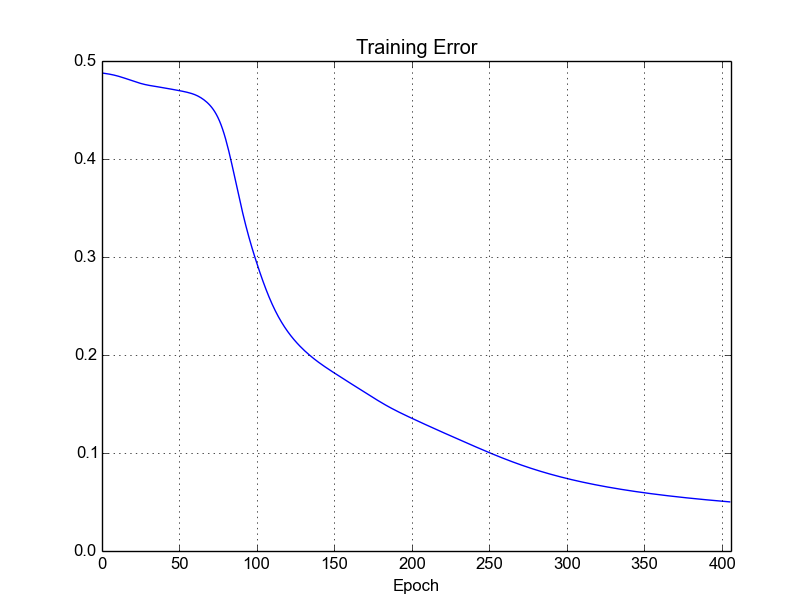
\includegraphics[width=\linewidth]{fig/trainingerror_lr0,0075_eps0,05_regparam0,00_beta5_batch1.png}
	\end{subfigure}
	\begin{subfigure}[b]{0.5\textwidth}
		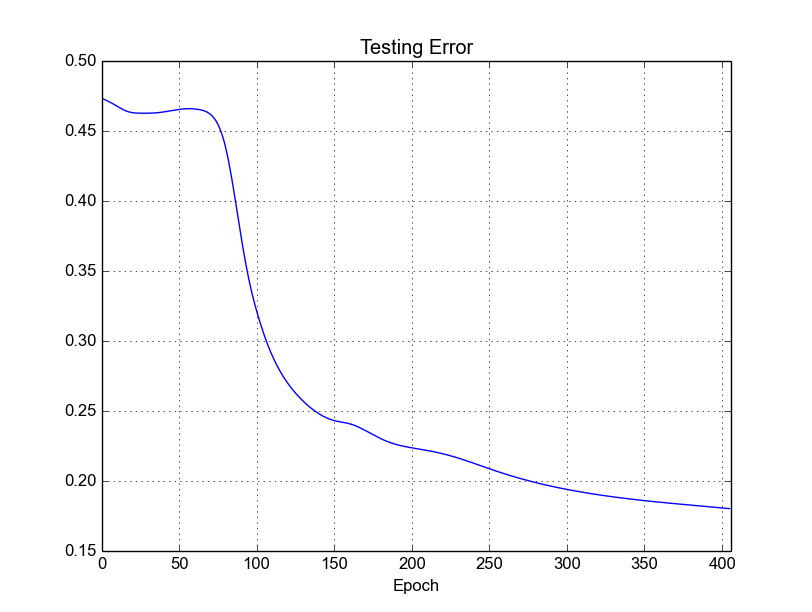
\includegraphics[width=\linewidth]{fig/valerror_lr0,0075_eps0,05_regparam0,00_beta5_batch1.png}
	\end{subfigure}

	\caption{\textbf{learning rate: 0.0075}}
\end{figure}



\begin{figure}[h]	
	\begin{subfigure}[b]{0.5\textwidth}
		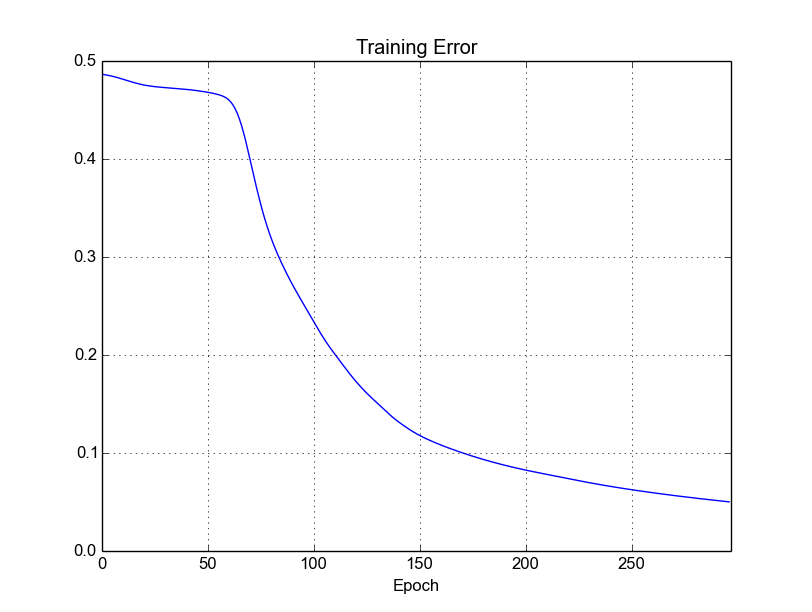
\includegraphics[width=\linewidth]{fig/trainingerror_lr0,01_eps0,05_regparam0,00_beta5_batch1.png}
	\end{subfigure}
	\begin{subfigure}[b]{0.5\textwidth}
		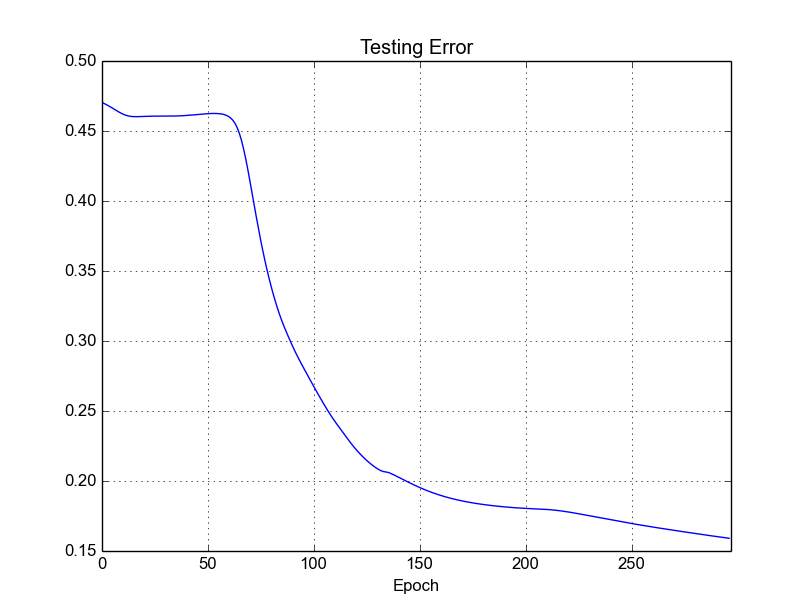
\includegraphics[width=\linewidth]{fig/valerror_lr0,01_eps0,05_regparam0,00_beta5_batch1.png}
	\end{subfigure}

	\caption{\textbf{learning rate: 0.01}}
\end{figure}


\begin{figure}[h]	
	\begin{subfigure}[b]{0.5\textwidth}
		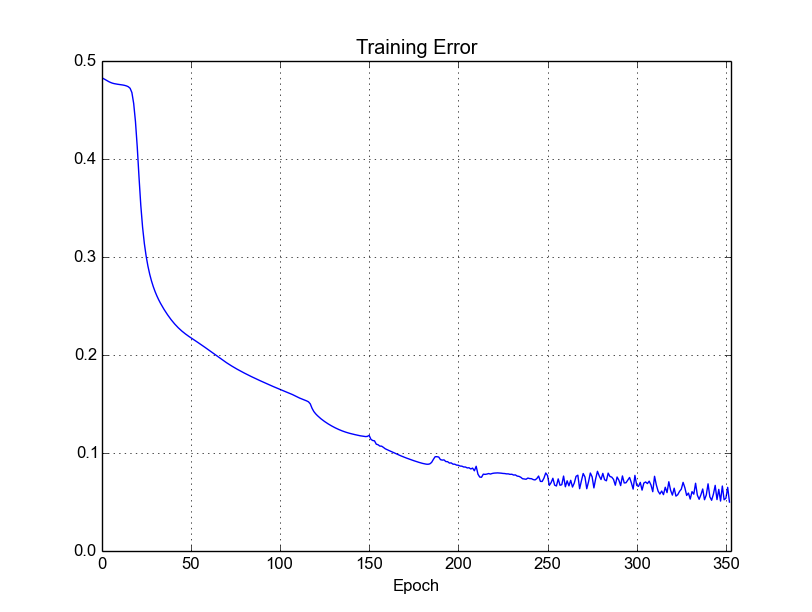
\includegraphics[width=\linewidth]{fig/trainingerror_lr0,025_eps0,05_regparam0,00_beta5_batch1.png}
	\end{subfigure}
	\begin{subfigure}[b]{0.5\textwidth}
		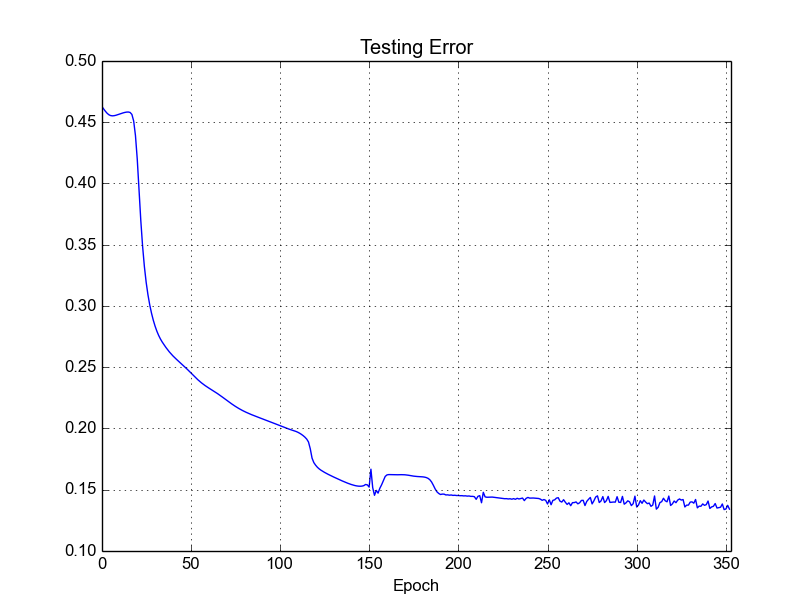
\includegraphics[width=\linewidth]{fig/valerror_lr0,025_eps0,05_regparam0,00_beta5_batch1.png}
	\end{subfigure}

	\caption{\textbf{learning rate: 0.025}}
\end{figure}



\begin{figure}[h]	
	\begin{subfigure}[b]{0.5\textwidth}
		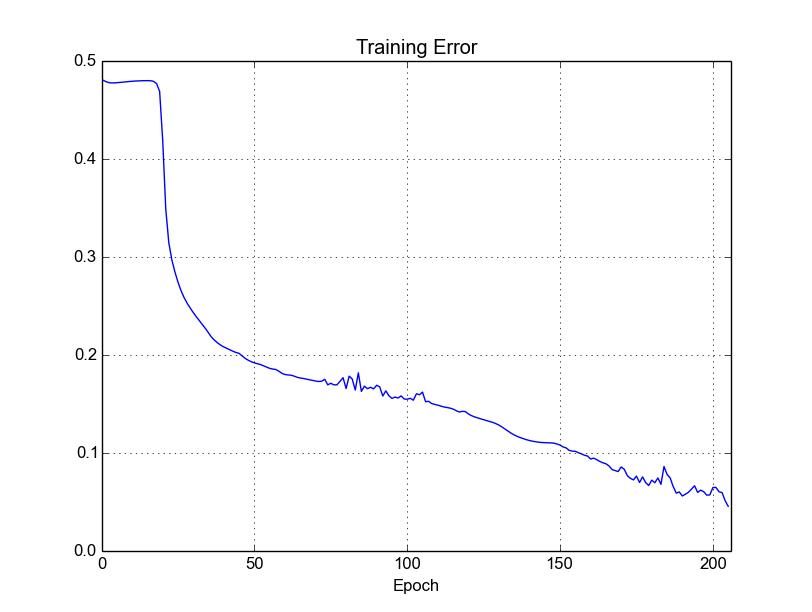
\includegraphics[width=\linewidth]{fig/trainingerror_lr0,05_eps0,05_regparam0,00_beta5_batch1.png}
	\end{subfigure}
	\begin{subfigure}[b]{0.5\textwidth}
		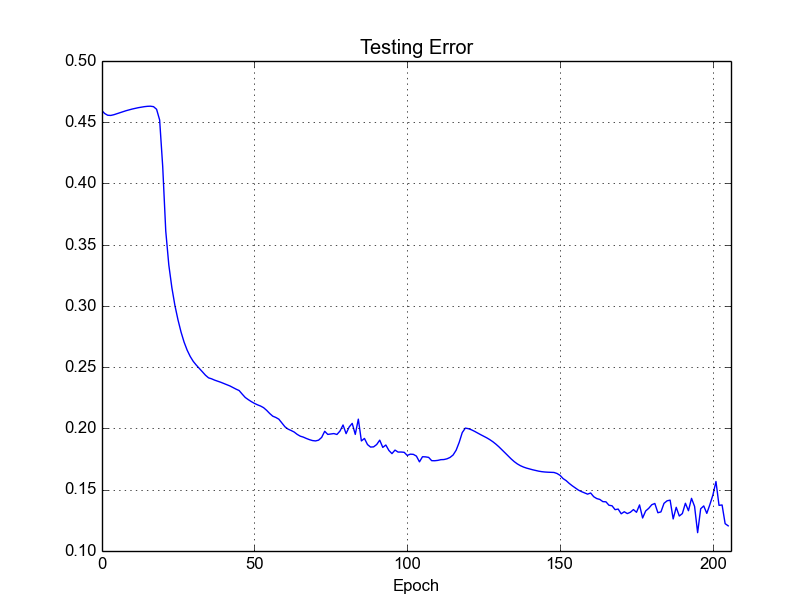
\includegraphics[width=\linewidth]{fig/valerror_lr0,05_eps0,05_regparam0,00_beta5_batch1.png}
	\end{subfigure}

	\caption{\textbf{learning rate: 0.05}}
\end{figure}


\subsubsection{Pruebas con distintos tamaños de mini batch}

Parámetros elegidos fijos:

\begin{itemize}
\item beta = 5
\item learning\_rate = 0.01
\item epochs = 1000
\item epsilon = 0.05
\item reg\_param = 0.0
\end{itemize}



\newpage
